\section{Results}\label{sec:results}

\subsection{Executor and Cost Model (E4)}
Thread adjustment acts on real parallelism. One partition reaches a speedup of \SpeedupSix{}
on the 6 physical cores and \SpeedupMax{} at \SpeedupMaxThreads{} threads, with no further
gain from simultaneous multithreading (\SpeedupTwelve{} at 12 threads). The cost
model~\eqref{eq:cost}, fitted on \CalPoints{} measured configurations, predicts held-out
configurations with $R^2=\CalRtwo$ and a mean absolute percentage error of \CalMape\%. This is
accurate enough to rank actions for the oracle labels. All headline results below use measured
time, not the model. The speedup curve and the fit are plotted in the artefact.


\subsection{Static Partition Quality (E1)}
Table~\ref{tab:e1} separates ACGR's contribution from that of the initial partitioner.
\begin{itemize}
  \item \emph{Repairing degraded partitions.} A partitioning that has absorbed many updates
        resembles a streaming (LDG) one. From LDG starts, ACGR reduces the edge cut by
        \EOnePubLDGCutRed\% on PubMed and \EOneCoraLDGCutRed\% on Cora (LP:
        \EOnePubLDGLPRed\% and \EOneCoraLDGLPRed\%). It obtains the lowest cut and CV of all
        refiners on the sparse graphs while staying within the 3\% balance tolerance.
  \item \emph{The CV term matters.} The cut-only ablation is no better than LP. The full
        objective lowers both CV and the cut.
  \item \emph{From METIS starts,} ACGR mainly trades cut for communication: CV falls by
        \EOnePubMetisCVRed\% on PubMed (cut change \EOnePubMetisCutRed\%).
  \item \emph{Limits.} METIS from scratch remains far better and is fast (\EOnePubMetisMs\,ms on
        PubMed). On the dense, power-law sx-mathoverflow graph, all local refiners gain little
        (\EOneMathLDGCutRed\% for ACGR from LDG). ACGR takes \EOnePubAcgrMs\,ms (PubMed, $k=8$),
        more than LP but small compared with an execution window.
\end{itemize}
Our first version reported a one-edge gain on Cora (744$\to$743). Its ACGR started from
Kernighan--Lin and penalised every imbalance. With the balance constraint and the CV term,
the same start yields the KL/ACGR rows of Table~\ref{tab:e1}.

\begin{table}[t]
\centering
\caption{Static partition quality, $k=8$, mean over 5 seeds: edge cut (\% of $|E|$),
communication volume (CV) and refinement time (ms).}\label{tab:e1}
\IfFileExists{tables/e1_quality_k8.tex}{\resizebox{\linewidth}{!}{\begin{tabular}{llrrrrrrrrrrrr}
\toprule
Initial & Refiner & \multicolumn{3}{c}{cora} & \multicolumn{3}{c}{pubmed} & \multicolumn{3}{c}{dblp} & \multicolumn{3}{c}{sx-mathoverflow} \\
 & & cut \% & CV & ms & cut \% & CV & ms & cut \% & CV & ms & cut \% & CV & ms \\
\midrule
METIS & none & 10.4 & 818 & -- & 11.8 & 6251 & -- & 5.7 & 280 & -- & 46.7 & 35839 & -- \\
METIS & LP & 10.2 & 812 & 0.7 & 11.7 & 6241 & 7.1 & 5.6 & 280 & 0.6 & 45.6 & 33932 & 10.8 \\
METIS & ACGR-cut & 10.2 & 812 & 1.6 & 11.7 & 6241 & 15.9 & 5.6 & 280 & 0.5 & 44.7 & 33440 & 87.2 \\
METIS & ACGR & 10.2 & 786 & 1.9 & 11.8 & 5994 & 22.5 & 5.6 & 274 & 0.9 & 44.9 & 33165 & 121.5 \\
\addlinespace
KL & none & 20.3 & 1626 & -- & 24.0 & 13114 & -- & 15.9 & 831 & -- & -- & -- & -- \\
KL & LP & 20.2 & 1615 & 0.7 & 23.3 & 12763 & 8.3 & 15.8 & 829 & 0.6 & -- & -- & -- \\
KL & ACGR-cut & 20.2 & 1615 & 2.2 & 23.3 & 12756 & 44.8 & 15.8 & 829 & 1.2 & -- & -- & -- \\
KL & ACGR & 19.8 & 1524 & 5.0 & 22.9 & 11958 & 55.9 & 15.3 & 790 & 2.6 & -- & -- & -- \\
\addlinespace
LDG & none & 38.7 & 2947 & -- & 45.7 & 24888 & -- & 30.4 & 1609 & -- & 74.4 & 56707 & -- \\
LDG & LP & 28.7 & 2255 & 0.9 & 30.9 & 16933 & 16.0 & 21.0 & 1101 & 0.8 & 72.4 & 54039 & 13.1 \\
LDG & ACGR-cut & 28.3 & 2239 & 6.8 & 30.5 & 16843 & 86.6 & 20.9 & 1102 & 3.2 & 72.6 & 54021 & 117.4 \\
LDG & ACGR & 24.5 & 1833 & 8.6 & 27.0 & 14249 & 97.4 & 18.3 & 927 & 3.8 & 72.8 & 53893 & 96.7 \\
\addlinespace
\bottomrule
\end{tabular}
}}{\RES{table missing}}
\end{table}

\subsection{Controller Quality (E2)}
The \NumSamples{} labelled states split into \LabelNO\% \NOA{}, \LabelTA\% \TA{}, \LabelRB\%
\RB{} and \LabelRP\% \RP{}. Table~\ref{tab:e2} reports decision quality on the
\NumTest{} test states from \NumTestGraphs{} unseen streams.
\begin{itemize}
  \item \emph{Learned versus rule-based.} The learned controllers reduce regret by about a
        quarter compared with the tuned threshold rule: GraphSAGE $\GSregret\pm\GSregretStd$\%,
        MLP $\MLPregret\pm\MLPregretStd$\%, threshold \THregret\%, never adapting \NOregret\%,
        always adjusting threads \TAallregret\%. Their macro-F1 is also higher (\GSFOne{} vs.\
        \THFOne). Always rebalancing (\RBallregret\%) or repartitioning (\RPallregret\%) is far
        worse, so firing the expensive actions at the wrong time is costly.
  \item \emph{What is learned.} Grid search sets the threshold rule's drift threshold to
        $\infty$, so it never rebalances. The GraphSAGE controller selects \RB{} in \GSPredRB\%
        of the states, with \GSRBprec\% precision and \GSRBrecall\% recall (Fig.~\ref{fig:e2}a).
        It never selects \RP{}: in \GSRPasRB\% of the states where global repartitioning is
        optimal, it chooses the cheaper local repair instead, which is a conservative choice
        given that a mistaken \RP{} costs \RPallregret\% on average. In the first iteration,
        trained without interaction streams, the controller selected neither \RB{} nor \RP{}
        (Sect.~\ref{sec:setup}). Selecting \RB{} on synthetic test states does not yet carry over
        to the real stream (E3).
  \item \emph{Ablations.} Message passing helps little: GraphSAGE and the MLP reach the same
        regret. With $k\le 8$, the communication graph is small and nearly complete, so pooling
        already exposes most of the information. Class-weighted cross-entropy performs
        similarly to the cost-sensitive loss ($\CEregret\pm\CEregretStd$\%).
\end{itemize}

\begin{figure}[t]
\centering
\IfFileExists{figs/e2_controller.pdf}{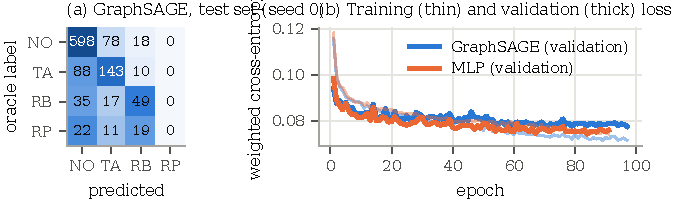
\includegraphics[width=\linewidth]{figs/e2_controller.pdf}}{\RES{figure missing}}
\caption{(a) Test confusion matrix of the GraphSAGE controller (NO: \NOA{}, TA: \TA{}, RB:
\RB{}, RP: \RP{}). (b) Loss curves of GraphSAGE and MLP (seed 0).}\label{fig:e2}
\end{figure}

\begin{table}[t]
\centering
\caption{Decision quality on held-out test graphs (mean $\pm$ std over 3 seeds). Regret is the
extra look-ahead cost $J_H(a)/J_H(a^\star)-1$ of the chosen action. Cost ratio is
$\sum J_H(a)/\sum J_H(a^\star)$.}\label{tab:e2}
\scriptsize
\IfFileExists{tables/e2_controller.tex}{\begin{tabular}{lcccc}
\toprule
Controller & Accuracy & Macro-F1 & Regret (\%) & Cost ratio \\
\midrule
GraphSAGE & 0.720 $\pm$ 0.011 & 0.469 $\pm$ 0.009 & 0.69 $\pm$ 0.07 & 1.0058 \\
MLP & 0.720 $\pm$ 0.002 & 0.453 $\pm$ 0.007 & 0.69 $\pm$ 0.02 & 1.0060 \\
Threshold (tuned) & 0.658 & 0.312 & 0.91 & 1.0079 \\
Never adapt & 0.638 & 0.195 & 1.20 & 1.0091 \\
Always \TA{} & 0.222 & 0.091 & 1.16 & 1.0086 \\
Always \RB{} & 0.093 & 0.042 & 8.51 & 1.0355 \\
Always \RP{} & 0.048 & 0.023 & 17.93 & 1.0859 \\
\bottomrule
\end{tabular}
}{\RES{table missing}}
\end{table}

\subsection{End-to-End Performance on Dynamic Graphs (E3)}
Table~\ref{tab:e3} reports measured end-to-end times on \NumScenarios{} scenarios
(2 streams $\times$ 2 values of $k$ $\times$ 3 platforms).
\begin{enumerate}
  \item \emph{Which adaptation pays depends on the workload.} On the hotspot-driven PubMed
        streams, thread reallocation gives the largest gains: Always-\TA{} is up to
        \SpPubEightSmAlwaysTA$\times$ faster than Static ($k=8$, SM), whereas periodic METIS is
        slower than Static (\SpPubEightSmPMETIS$\times$) because it migrates many vertices for
        little structural gain. On the steadily drifting real stream, periodic global
        repartitioning is the best deployable policy (\SpMathFourOnePMETIS$\times$ at $k=4$ on
        1\,GbE; Oracle \SpMathFourOneOracle$\times$), and thread reallocation adds little
        (\SpMathFourOneAlwaysTA$\times$).
  \item \emph{The learned controllers perform on par with simple heuristics, not better.}
        No fixed heuristic is best everywhere: periodic METIS is up to \RobPMETISMax\% and
        Always-\TA{} up to \RobAlwaysTAMax\% behind the best deployable policy of a scenario.
        GraphSAGE is behind by \RobGSAGEMean\% on average (worst case \RobGSAGEMax\%), slightly
        more than Always-\TA{} (\RobAlwaysTAMean\%) and the threshold rule
        (\RobThresholdMean\%), and similar to the MLP (\RobMLPMean\%). It beats Static in
        \FasterGSAGE{} of the \NumScenarios{} scenarios, significantly in \SigFasterGSAGE{}. On
        the real stream at $k=8$, all thread-adjusting policies are marginally slower than
        Static. Its controller overhead is \CtrlGSAGE\% of the total time, and it is not the
        best policy in any scenario.
  \item \emph{The gap to the Oracle is global repartitioning.} On sx-mathoverflow the Oracle
        chooses \RB{} \MathRBOracle{} times and \RP{} \MathRPOracle{} times. The learned
        controllers trigger neither action on the evaluation streams, although they select \RB{}
        on synthetic test states (E2).
  \item \emph{Speculative or unconditional repartitioning does not pay.} MPC must run ACGR and
        METIS in every window to evaluate them, and is slower than Static in every scenario
        (e.g.\ \SpPubEightSmMPC$\times$). This is the main argument for a millisecond-scale
        learned or rule-based trigger. Always-ACGR is slower than Static except on the real
        stream with $k=4$ on 1\,GbE (\SpMathFourOneAlwaysACGR$\times$).
\end{enumerate}

\begin{table}[t]
\centering
\caption{End-to-end time $J$ (s): sum of per-window median times plus overheads (mean over
seeds for PubMed). Bold: best deployable policy. $^{*}$: $p<0.05$ versus Static (paired
Wilcoxon on per-window times, all seeds).}\label{tab:e3}
\IfFileExists{tables/e3_totals.tex}{\resizebox{\linewidth}{!}{\begin{tabular}{lllrrrrrrrrr}
\toprule
Stream & $k$ & Platform & Static & Always-TA & Always-ACGR & P-METIS & Threshold & MPC & MLP & GraphSAGE & Oracle \\
\midrule
PubMed-synthetic & 4 & sm & 1.05 & \textbf{0.97} & 1.34$^{*}$ & 1.21 & 0.98 & 3.24$^{*}$ & 1.00 & 1.00 & 1.02 \\
PubMed-synthetic & 4 & 10g & 1.54 & \textbf{1.46} & 1.86$^{*}$ & 1.71 & 1.47 & 3.70$^{*}$ & 1.49 & 1.49 & 1.52 \\
PubMed-synthetic & 4 & 1g & 3.12 & \textbf{3.04} & 3.75$^{*}$ & 3.51 & 3.05 & 5.59$^{*}$ & 3.08 & 3.08 & 2.99$^{*}$ \\
PubMed-synthetic & 8 & sm & 1.33 & \textbf{1.07}$^{*}$ & 1.57 & 1.61 & 1.08$^{*}$ & 3.80$^{*}$ & 1.11 & 1.11 & 1.10$^{*}$ \\
PubMed-synthetic & 8 & 10g & 3.26 & \textbf{3.00}$^{*}$ & 3.49 & 3.54 & 3.02$^{*}$ & 5.74$^{*}$ & 3.03$^{*}$ & 3.04$^{*}$ & 3.03$^{*}$ \\
PubMed-synthetic & 8 & 1g & 7.20 & \textbf{6.94}$^{*}$ & 7.50$^{*}$ & 7.54 & 6.95$^{*}$ & 9.60$^{*}$ & 6.96$^{*}$ & 6.97$^{*}$ & 6.81$^{*}$ \\
sx-mathoverflow & 4 & sm & 4.44 & 4.15$^{*}$ & 4.61$^{*}$ & \textbf{3.93}$^{*}$ & 4.17$^{*}$ & 7.11$^{*}$ & 4.20$^{*}$ & 4.28$^{*}$ & 3.88$^{*}$ \\
sx-mathoverflow & 4 & 10g & 6.04 & 5.75$^{*}$ & 6.19$^{*}$ & \textbf{5.39}$^{*}$ & 5.78$^{*}$ & 8.17$^{*}$ & 5.80$^{*}$ & 5.80$^{*}$ & 5.35$^{*}$ \\
sx-mathoverflow & 4 & 1g & 17.56 & 17.27$^{*}$ & 16.99$^{*}$ & \textbf{15.61}$^{*}$ & 17.30$^{*}$ & 18.08 & 17.31$^{*}$ & 17.32$^{*}$ & 15.15$^{*}$ \\
sx-mathoverflow & 8 & sm & 4.93 & 5.01$^{*}$ & 5.91$^{*}$ & \textbf{4.79} & 4.98 & 8.33$^{*}$ & 4.99 & 5.00 & 4.80$^{*}$ \\
sx-mathoverflow & 8 & 10g & 8.53 & 8.61$^{*}$ & 9.55$^{*}$ & \textbf{8.31} & 8.57 & 12.03$^{*}$ & 8.58 & 8.59 & 8.26$^{*}$ \\
sx-mathoverflow & 8 & 1g & 27.46 & 27.54$^{*}$ & 28.60$^{*}$ & \textbf{26.27}$^{*}$ & 27.50 & 29.18$^{*}$ & 27.53 & 27.53 & 25.59$^{*}$ \\
\bottomrule
\end{tabular}
}}{\RES{table missing}}
\end{table}

\subsection{Discussion and Recommendations}
\begin{itemize}
  \item \emph{Transient imbalance} (hotspots) is best handled by thread reallocation. It
        costs about a millisecond, migrates nothing, and should be applied whenever thread
        pressure is uneven. Learned and rule-based triggers both do this reliably.
  \item \emph{Persistent structural drift} requires repartitioning. ACGR repairs sparse graphs
        cheaply (E1). On the dense real stream only global repartitioning helps, and it pays off
        on all three platforms.
  \item \emph{Learned control} has the lowest per-decision regret, but end to end it matches
        simple heuristics and does not exploit repartitioning on the evaluation streams. Our
        practical recommendation is a cheap thread-adjustment trigger combined with periodic or
        drift-triggered global repartitioning. Learning \emph{when to repartition globally}
        remains open: on the real stream GraphSAGE is up to \RobOracleGap\% slower than the
        Oracle.
\end{itemize}
\paragraph{Limitations.} We measure on one 6-core laptop and emulate networks analytically.
The cost model must be recalibrated for each machine, and the look-ahead assumes \NOA{} after
the first action. The dynamic experiments use one real temporal graph and $k\le 8$.
